\documentclass[a4paper, 12pt, svgnames]{article}

\usepackage{preambule}
\newcommand{\mr}[1]{{\textcolor[rgb]{0.80,0.10,0.1}{#1}}}

\title{Variabilités intrinsèques des SNe Ia et leurs conséquences sur les
paramètres cosmologiques}

\fancyhead[L]{\scriptsize \textsc{Variabilités intrinsèques des SNe Ia}}

\begin{document}

\thispagestyle{empty}
\noindent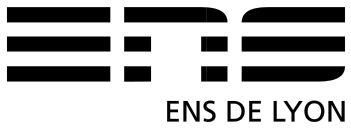
\includegraphics[height=2cm]{General_figures/logoens.png} \hfill

\includegraphics[height=2cm]{General_figures/logoucbl.png} \hfill

\includegraphics[height=2cm]{General_figures/logounivlyon.png}\vfill

\noindent\begin{tabularx}{\linewidth+27pt}{@{} l X r @{} }
{\textsc{Master Science de la matière}} & & Année 2018--2019\hspace*{1cm}\\
{\textit{École Normale Supérieure de Lyon}} & & \textsc{Nicolas} Nora\hspace*{1cm}\\
{\textit{Université Claude Bernard Lyon I}} & & M2 Physique\hspace*{1cm}
\end{tabularx}

\begin{center}\vfill\hrule\vspace*{8pt}

\textbf{\huge Variabilités intrinsèques des SNe Ia et leurs conséquences sur les
paramètres cosmologiques}\\

\hrule\vfill

\parbox{15cm}{\small\textbf{Résumé}:
L'étude des supernovae de type Ia a de nombreuses utilités en physique. Elle
sert notamment à la détermination de paramètres cosmologiques, comme la
constante de Hubble ou le paramètre d'état de l'énergie noire. Afin d'améliorer
la précision et la justesse des mesures existantes, les incertitudes
statistiques et systématiques doivent être traitées correctement. Si l'ajout de
données permet de réduire les incertitudes statistiques, il n'y a que l'étude du
comportement physique des supernovae qui permet de réduire les incertitudes
systématiques. Dans ce rapport, nous discutons comment l'établissement de lois
d'évolution du paramètre de durée d'explosion d'une supernova en fonction du
redshift permettrait d'atteindre ce but.}\vspace{0.5cm}

\parbox{15cm}{\small\textbf{Mots-clés}:
Cosmologie, supernovae}\vspace{0.5cm}

\parbox{15cm}{Stage supervisé par:\\
\textbf{\textsc{RIGAULT} Mickaël}, Chercheur\\
\href{mailto:rigault@ipnl.in2p3.fr}{rigault@ipnl.in2p3.fr}\\
\href{https://www.ipnl.in2p3.fr/perso/rigault/}{Site personnel}\bigbreak
Institut de Physique des Deux Infinis\\
{\textit{Université Lyon 1\\4 rue Enrico Fermi -- bâtiment Dirac\\
69622 Villeurbanne Cedex}}\\
\url{https://www.ipnl.in2p3.fr}}\vspace{.5cm}\vfill

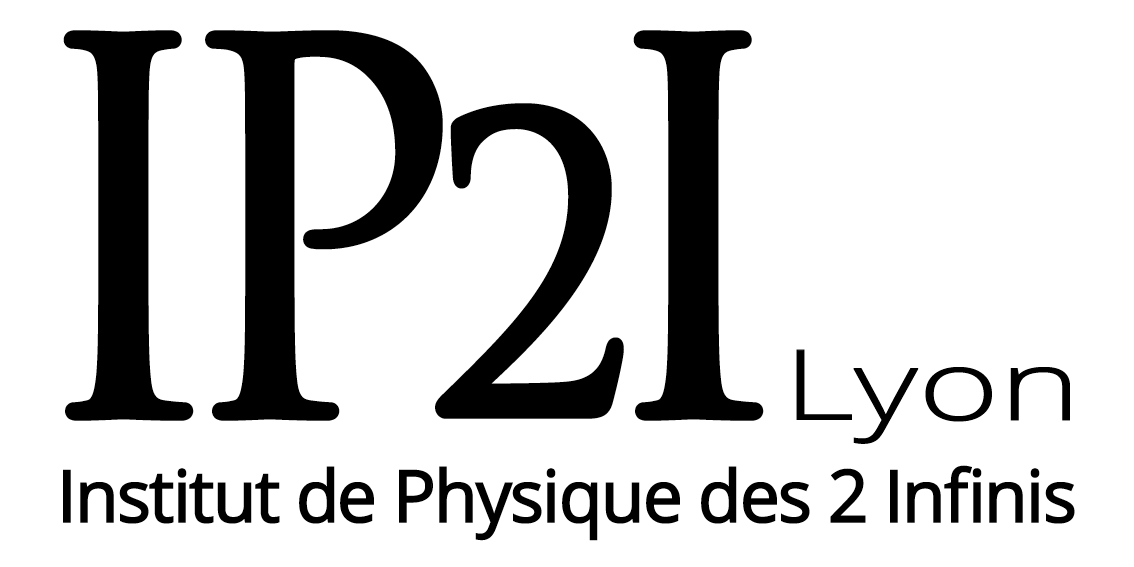
\includegraphics[width=.3\textwidth]{General_figures/IP2I.png}
\end{center}\vfill \hfill \today
\newpage
\thispagestyle{empty}
\setcounter{page}{0}

\appsec{Remerciements}{sec:ack}

Je tiens à remercier toutes les personnes qui ont contribué, de près ou de loin,
à la réalisation de ce stage et de ce rapport de stage. En premier lieu, bien
évidemment, je remercie Mickaël \bsc{Rigault} pour son encadrement sans faille

\tableofcontents
\newpage

\section{Introduction}\label{sec:int}

En cosmologie, l'étude des supernovae de type Ia (SNe~Ia) permet de mesurer
l'histoire de l'expansion de l'univers et ainsi d'étudier la physique des
éléments fondamentaux qui le composent, et notamment celle de l'énergie noire
\cite{perlmutter_measurements_1999, riess_observational_1998}. Avec aujourd'hui
$\approx1000$ SNe~Ia, les incertitudes systématiques commencent à dominer le
budget d'erreur lors de la mesure des paramètres cosmologiques
\cite{betoule_improved_2014, scolnic_complete_2018}. Parmi celles-ci, l'un des
effet dominant est lié à notre connaissance limitée de la physique même des
SNe~Ia~\cite{sullivan_dependence_2010, rigault_evidence_2013,
rigault_confirmation_2015}.

La cosmologie avec les SNe~Ia repose sur le fait qu'il est possible de prédire
leur luminosité à toutes distance de nous, et donc à tout moment dans le passé.
Les SNe~Ia sont ainsi supposées être des chandelles standards (ou plutôt
standardisables, nous le verrons) de la cosmologie. Cependant, la physique des
étoiles change avec l'histoire de l'univers : serait-il alors possible que la
physique des SNe~Ia change également ? Si oui, est-ce que cela pourrait impacter
la détermination des paramètres cosmologiques ? et de combien ?

Dans ce rapport, nous étudions un paramètre intrinsèque à la physique
de l'explosion du progéniteur en SNe~Ia : l'étallement de la courbe de lumière,
dit ”stretch” \mr{phillips199?}, et nous nous intéressons à son évolution
potentielle en fonction de l'âge de l'univers. Si nous trouvons qu'il évolue,
alors nous aurons déterminé que la physique des SNe~Ia change en fonction du
temps comme suggéré par
\cite{howell_effect_2009, rigault_evidence_2013, childress_ages_2014,
rigault_strong_2018}.

\mr{ICI PRESENTATION DU PLAN. Nous commencerons section~\ref{sec:cosmo} par
présenter la cosmologie avec les SNeIa en revenant sur le concept de chandelles
standard(isable)s et la détermination des paramètres cosmologiques.
BLABLABLA...}

\section{Cosmologie avec les Supernovae de type Ia}\label{sec:cosmo}
\subsection{Chandelles standards et diagramme de Hubble}\label{ssec:hub}

En astronomie, la mesure d'un flux lumineux (F) est généralement exprimé en
magnitude (m), tel que :

\begin{equation}
    m - m_0 = -2.5\log\LR{F}{F_0},
\end{equation}

où $m_0$ ($F_0$) représente une magnitude (flux) de référence.
Le flux étant relié à la luminosité $L$ d'une source lumineuse à la distance
$d_L$ par $F = L\times \left(4\pi d_L²\right)^{-1}$, on a alors :

\begin{equation}
    m - m_0 = -2.5\log\LR{L}{4\pi d_L²} + C.
\end{equation}

La magnitude $m$, dite « apparente », dépend donc de la distance. On définit
la magnitude \textit{absolue} -- liée cette fois à la luminosité intrinsèque du
corps observé -- comme la magnitude apparente qu'aurait la source si elle était
située à une distance de $\SI{10}{pc}$ :

\begin{equation}
    M = -2.5\log\LR{L}{4\pi\LF{\SI{10}{pc}}²} + C
\end{equation}

On peut alors définir le \textit{module de distance} $\m$ qui représente la
distance de la source par :

\begin{equation}
    \m \equiv m - M = 5\log(d_L) - 5
\end{equation}
avec $d_L$ en parsec. 

En considérant un univers plat homogène et isotrope, l'équation de
\bsc{Friedmann}-\bsc{Lemaître} mène à une expression de $d_L$ dépendant des
paramètres cosmologiques d'après la relation

\begin{equation}\label{dL}
    d_L = \LF{1 + z} \times c \LF{ \int_0^z \d z' \left[ \O_R
    \LF{1 + z'}⁴ + \O_M \LF{1 + z'}³ + \O_{\L} \right]^{-1/2}},
\end{equation}

avec $\O_R$ la densité d'énergie de rayonnement, $\O_M$ la densité d'énergie de
matière, et $\O_\L$ la densité d'énergie noire. Pour un univers plat elles sont
reliées par la relation

\begin{equation}
    1 = \O_R + \O_M + \O_\L.
\end{equation}

Ainsi, le module de distance $\m$ permet de de déterminer $d_L$ \textit{via} la
mesure de la magnitude apparente $m$, si la magnitude absolue $M$ est connue.
On appelle « chandelle standard » un objet dont $M$ est ainsi prédictible.
Remarquez que pour des mesures de distances relatives, $M$ n'as pas besoin
d'être connu absolument, mais simplement d'être le même entre les objets que
nous comparons. Les SNe~Ia sont de telles objets et sont également extrêmement
brillantes ce qui nous permet de faire des mesures de distances à l'échelle
cosmologique (milliards d'années lumière).

\subsection{Les SNe~Ia}\label{ssec:sneia}
Si les SNe~Ia sont considérées comme des chandelles standards, c'est parce
qu'elles obéissent au même mécanisme d'explosion. Bien qu'il soit encore mal
compris, on sait qu'il résulte de l'augmentation de la masse de naines
blanches, des étoiles inertes très denses, qui mènerait à une explosion
thermonucléaire lorsqu'elles atteignent la masse critique de \bsc{Chandrasekhar}
de \SI{1.4}{M_\odot}. Cette augmentation peut suivre de l'accrétion d'un
compagnon qui est généralement une géante rouge, ou par fusion de deux naines
blanches.

Elles sont beaucoup étudiées en cosmologie de fait de leur forte luminosité
permettant une mesure de magnitude jusqu'à des redshifts de l'ordre de $z
\approx 1$, ce qui équivaut à une analyse des propriétés cosmologiques de
l'Univers quand il était de la moitié de son âge actuel. Elles sont notamment
les meilleures candidates pour les études à bas redshift, leur luminosité (sur
une courte période) pouvant dépasser celle de leur galaxie hôte contenant des
centaines de milliards d'étoiles,  et qui, d'après l'équation \ref{dL}, est la
zone d'Univers où le paramètre d'énergie noire domine (pour $z \leq 1$, c'est le
terme en $\O_\L$ qui domine étant donné la puissance $-1/2$ sur le crochet). Un
des buts de l'utilisation des SNe Ia en cosmologie est de mieux comprendre le
comportement de cette énergie noire, sa densité précise et l'évolution de sa
densité.

Mais en réalité, il existe une dispersion naturelle d'environ 40\% des
magnitudes absolues des SNe~Ia. Elles ne sont donc pas parfaitement standards et
cette dispersion correspond une imprécision de $\approx 20\%$ sur la valeur de
la distance déduite. Cependant, il existe des relations empiriques qui
permettent de réduire cette dispersion d'un facteur trois, ce qui en en fait
l'un des outils de mesure de distances le plus précis en astronomie.

\subsection{Courbes de lumière}\label{ssec:lc}

Les SNe~Ia sont des objets astronomiques dit transitoires : leur flux évolue en
fonction du temps. La forme de cette évolution dépend de la physique intrinsèque
à l'explosion du progéniteur -- les éléments radioactifs créés et détruits
notamment. Les éléments extrinsèques, notamment les milieux interstellaires de
la galaxie hôte et de notre propre galaxie, eux, peuvent affecter la luminosité
relative entre les gammes de longueurs d'onde observées -- les poussières
interstellaires absorbent plus dans le bleu que dans le rouge, faisant paraître
les objets plus rouges qu'ils ne le sont. On appelle « courbe de lumière »
l'évolution de la luminosité d'un objet en fonction du temps. La
figure~\ref{fig:lightcurves} montres les courbes de lumière d'une SNe~Ia
(SN2011fe) dans cinq bandes spectrales \cite{pereira_spectrophotometric_2013}.

\begin{figure}[htbp!]
    \centering
    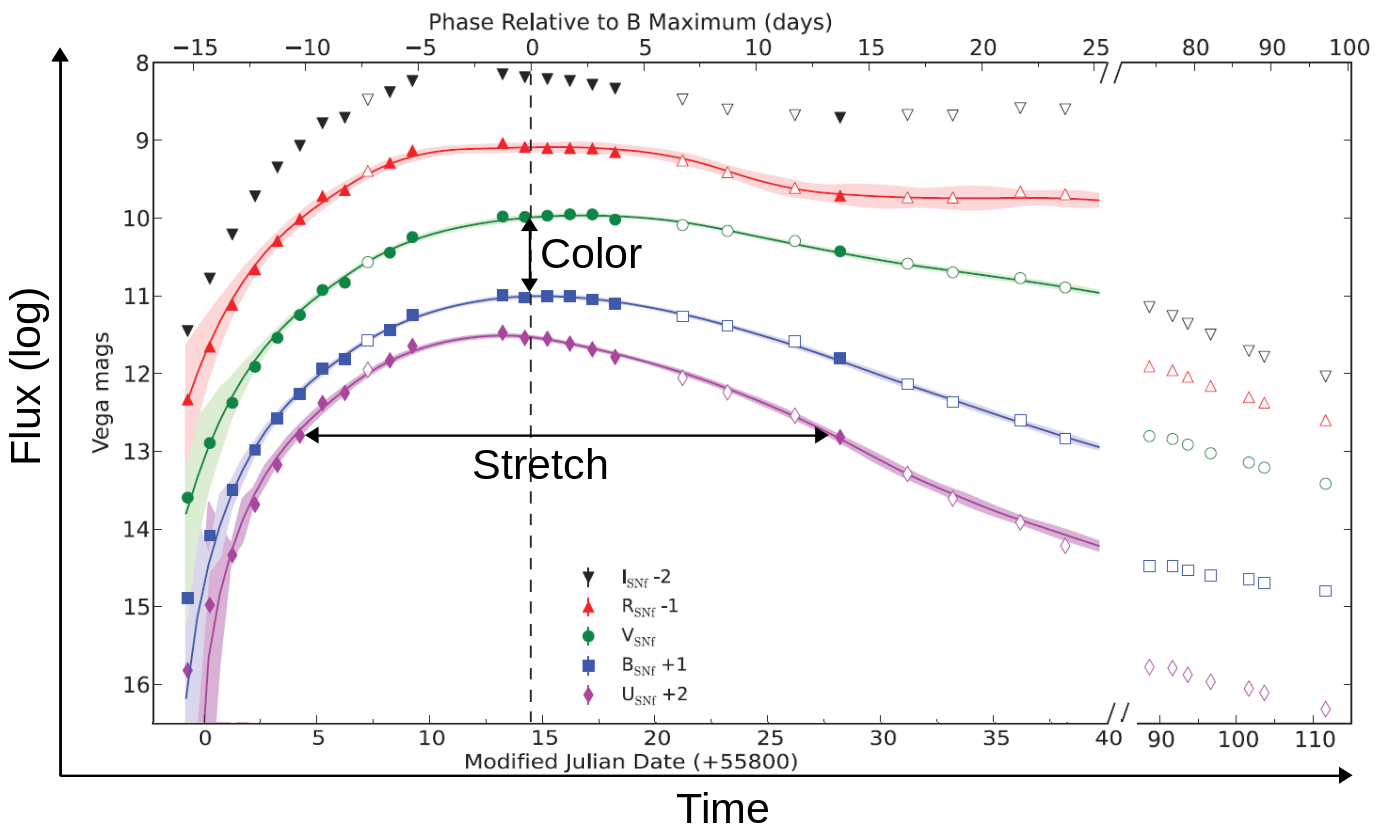
\includegraphics[width=.5\linewidth]{Rapport_figures/lightcurve.png}
    \captionsetup{justification=centering}
    \caption{Exemple de courbe de lumière d'une supernova depuis son explosion
    pour différentes longueurs d'ondes. On peut y définir un paramètre de
couleur et un paramètre de \textit{stretch} qui estime la durée d'explosion de
ladite SNe Ia.}
    \label{fig:lightcurves}
\end{figure}

Ainsi, la chandelle standard de la SNe~Ia est en réalité définie comme sa
luminosité dans la bande bleue ($\approx5000\A$) à son maximum de luminosité.

Les courbes de lumières des SNe~Ia sont paramétrisées par trois éléments :

\begin{enumerate}
    \item Le maximum de luminosité dans la bande B, il s'agit du « $m$ des
        SNe~Ia » ;
    \item La couleur (« c »), définie par la différence de magnitude au maximum
        d'émission entre les bandes vertes et bleues ;
    \item Le \textit{stretch} (« $x_1$ »), définissant l'élargissement de la
        courbe de lumière.
\end{enumerate}

L'algorithme SALT2~\cite{guy_salt2_2007, guy_supernova_2010} permet d'ajuster
ces paramètres.

\begin{figure}[htbp!]
    \centering
    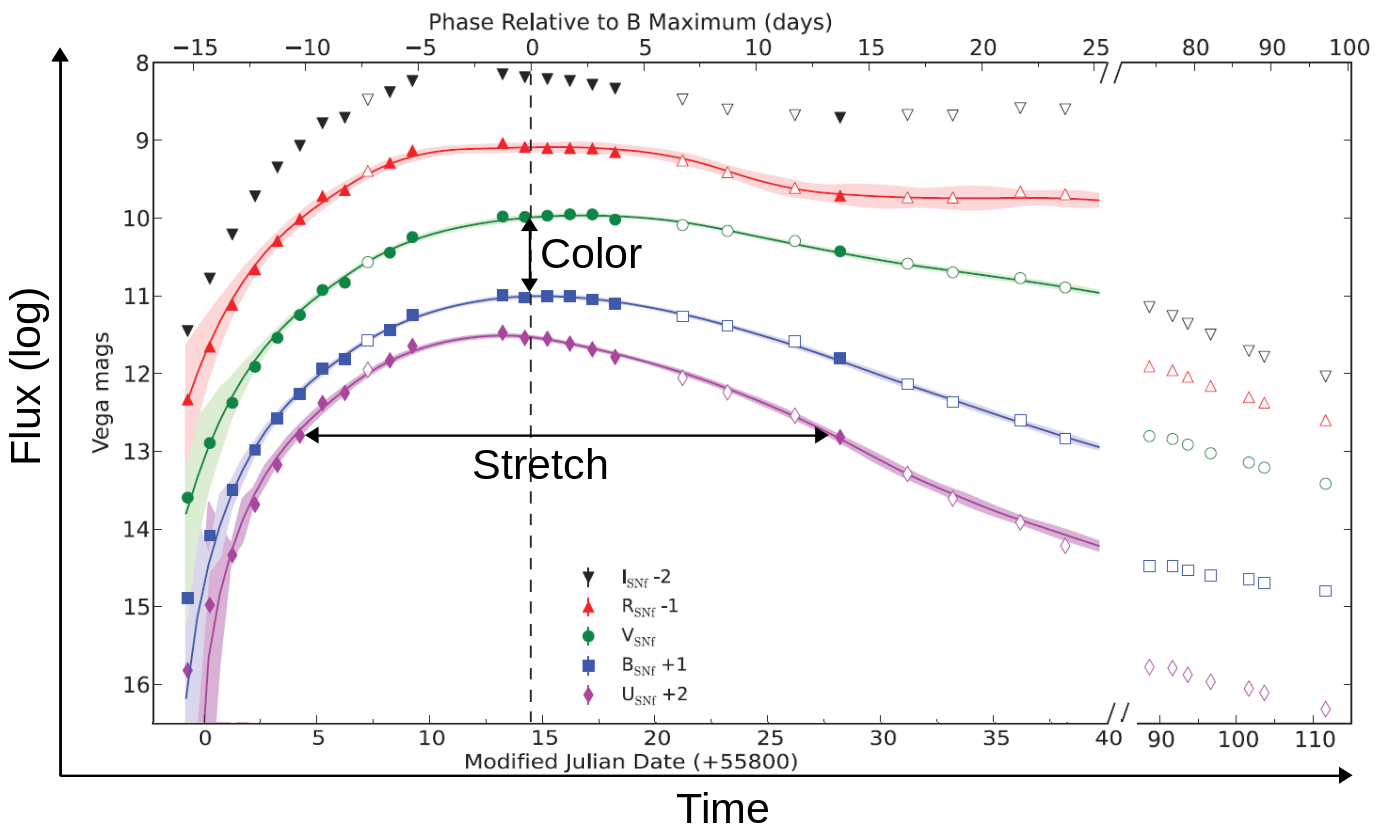
\includegraphics[width=.5\linewidth]{Rapport_figures/lightcurve.png}
    \captionsetup{justification=centering}
    \caption{Exemple de courbe de lumière d'une supernova depuis son explosion
    pour différentes longueurs d'ondes. On peut y définir un paramètre de
couleur et un paramètre de \textit{stretch} qui estime la durée d'explosion de
ladite SNe Ia.}
    \label{lightcurves}
\end{figure}

La définition de ces paramètres n'est pas anodine : il existe une corrélation
entre $M_B$ (la magnitude absolue des SNe~Ia dérivée de $m_B$) et le stretch
$x_1$ et la couleur $c$ (mais pas entre $x_1$ et $c$ par construction). Les
SNe~Ia à évolution lente (grand stretch) ont une luminosité intrinsèque plus
grande (relation "brighter-slower") \mr{phillips199?} et les SNe~Ia les plus
bleues sont plus lumineuses (relation "brighter-bluer") \mr{tripp199?,
Riess1996}. Ces relations sont illustrées figure \ref{brighter_slower_bluer}.

\begin{figure}[htbp!]
    \centering
    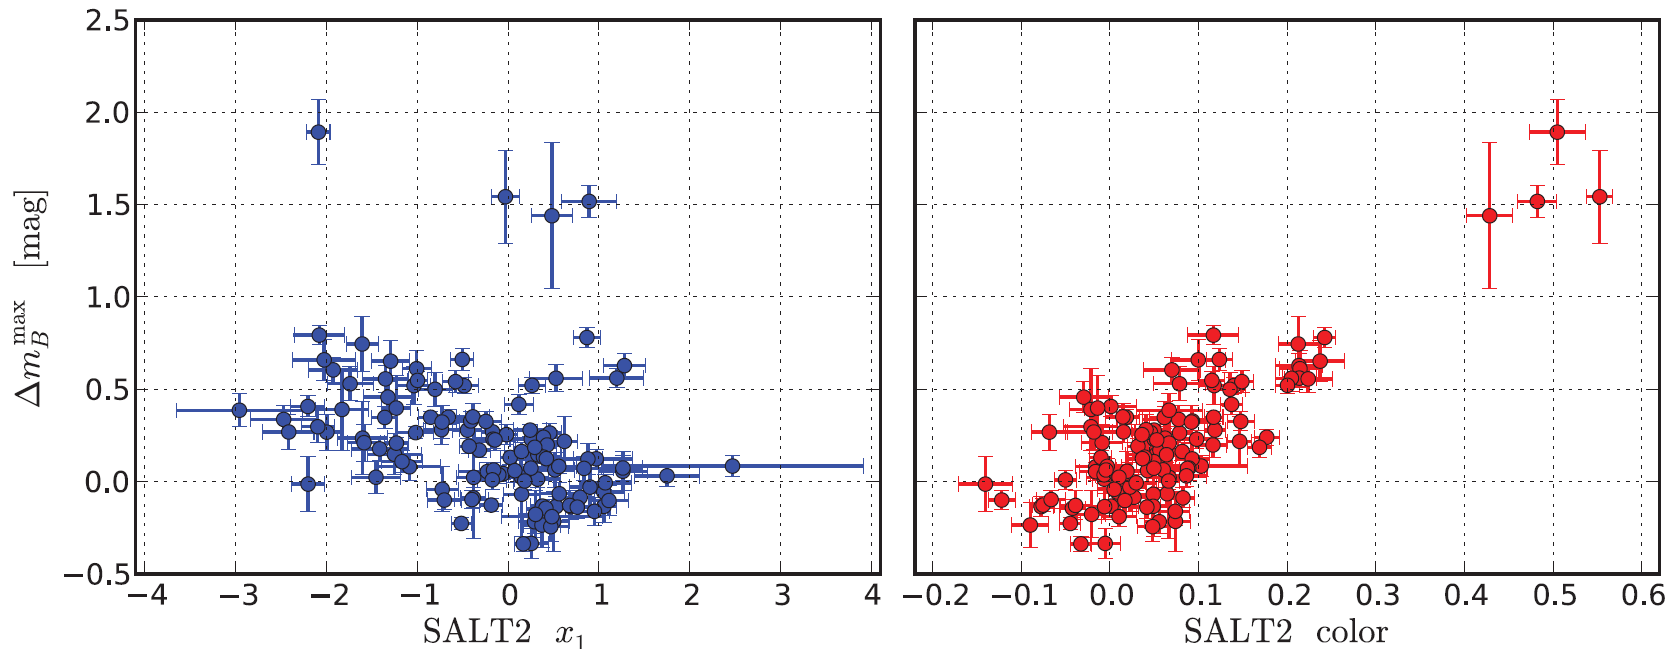
\includegraphics[width=.7\linewidth]{Rapport_figures/disp_x1_c.PNG}
    \captionsetup{justification=centering}
    \caption{Corrélations entre la différence de luminosité maximale d'une
    supernova dans le bleu et les paramètres de stretch (« $x_1$ ») et de
couleur (« color ») d'après l'algorithme SALT2.}
    \label{brighter_slower_bluer}
\end{figure}

Pour réduire la dispersion naturelle de magnitude absolue des SNeIa, on peut
alors inclure ces relations linéaires dans l'expression de la magnitude absolue,
de telle sorte que :

\begin{equation}
    M_B{}^{\text{corr}} \equiv M_B{}^{\text{max}} + \LF{\a x_1 - \b c}
\end{equation}

où $\a$ est le coefficient du stretch, et $\b$ celui de la couleur, tous les
deux positifs ; $M_B{}^{corr}$ est la nouvelle définition de la magnitude
absolue des SNeIa, dite « standardisée ». Ces trois paramètres sont ajustés
simultanément sur l'ensemble des données disponibles.

Ces relations supplémentaires permettent de réduire l'incertitude sur la
mesure de distance, puisque la dispersion de magnitude absolue est réduite à
$\approx 0.15 \mathrm{mag}$ \cite{betoule_improved_2014}, soit une précision en
distance de l'ordre de 8\%. La nouvelle définition du module de distance
(standardisé) des SNeIa est :

\begin{equation}
    \m = m - M +\a x_1 - \b c
\end{equation}

La réduction de la dispersion dans le diagramme de Hubble est illustré
\ref{disp_20} avec les données de SNfactory \cite{rigault_strong_2018}.

\begin{figure}[htbp!]
    \centering
    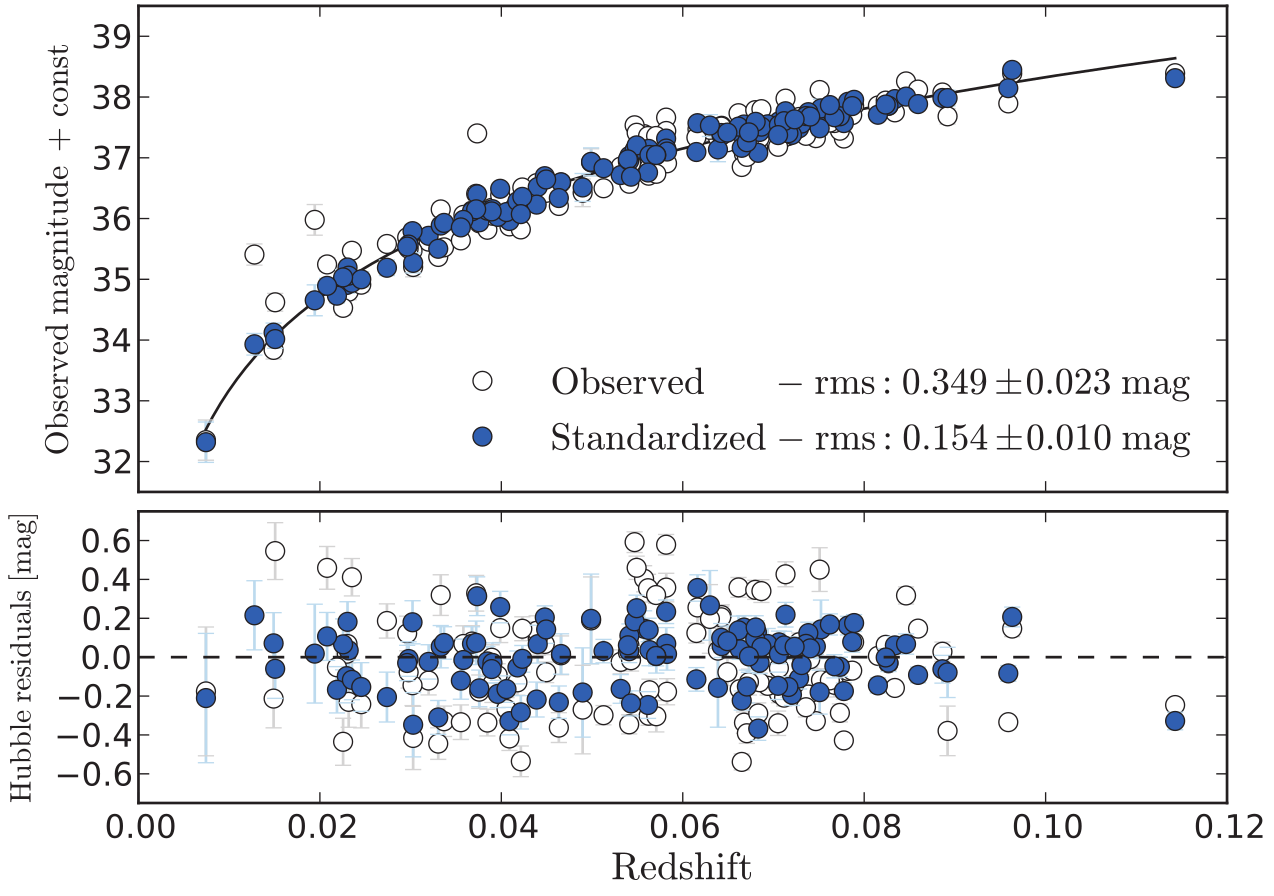
\includegraphics[width=.5\linewidth]{Rapport_figures/disp_beau.png}
    \captionsetup{justification=centering}
    \caption{Diagramme de Hubble avec, en haut, la magnitude apparente avant et
        après le processus de standardisation, qui consiste à inclure les
        corrélations entre la magnitude absolue et les paramètres de stretch et
        de couleur, respectivement en blanc et en bleu. En bas, on a le
        \textit{résidu} ne montrant que la dispersion autour de la courbe noire,
        indiquant l'évolution de la luminosité prédite par la loi de Hubble.}
    \label{disp_20}
\end{figure}

L'utilisation de cette relation a alors permis d'améliorer la précision des
mesures de distance, et ainsi discriminer différentes valeurs possibles pour les
paramètres cosmologiques : cela a mené à la découverte de l'expansion accélérée
de l'Univers \textit{via} une valeur non-nulle de $\O_\L$ pour laquelle un prix
Nobel a été descerné en 2011. La dernière compilation des SNe~Ia est
présentée fig~\ref{hub_acc_exp} [\mr{METTRE CELLE DE SCOLNIC}].

\begin{figure}[htbp!]
    \centering
    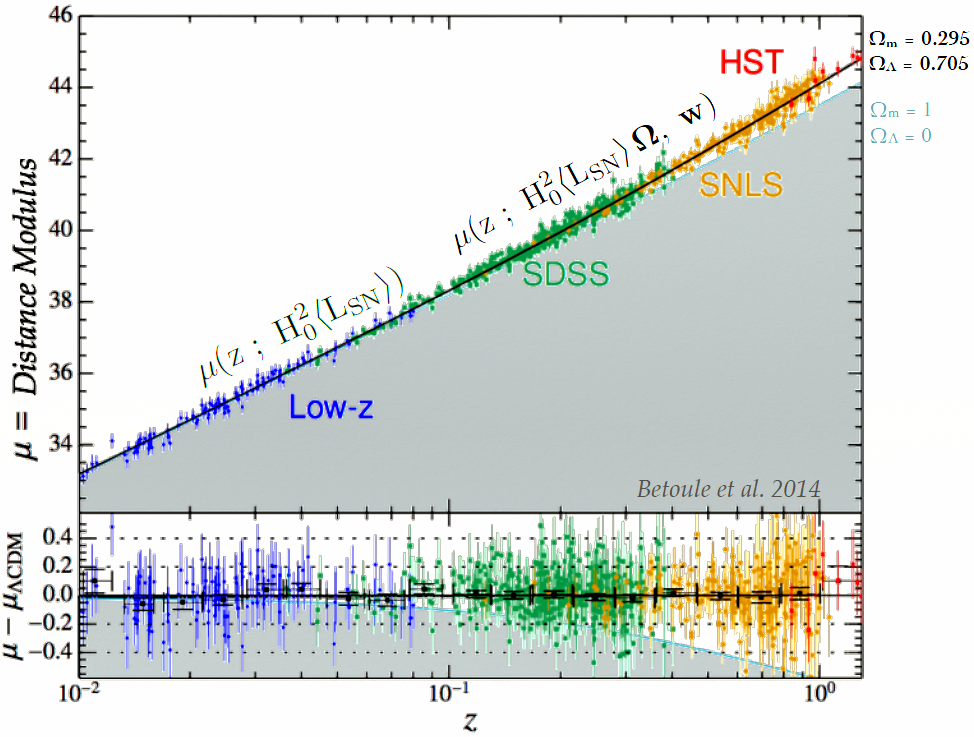
\includegraphics[width=.5\linewidth]{Rapport_figures/bet_al_2.PNG}
    \captionsetup{justification=centering}
    \caption{Diagramme de Hubble actuel (en couleurs, une par échantillon
             d'observation) comparé au diagramme de Hubble avant la découverte 
             de l'expansion accélérée de l'Univers (en gris) en haut, et
             diagramme résiduel où l'on a retiré l'évolution théorique du module
             de distance.}
    \label{hub_acc_exp}
\end{figure}

\subsection{Incertitudes systématiques}\label{ssec:syst}

Depuis la découverte de l'accélération de l'expansion de l'univers, qui ne se
basait que sur une centaine de données de SNe Ia, plus de données ont été
accumulées, et la précision sur les mesures de $\O_M$ et $\O_\L$ s'est
améliorée. Nous pouvons maintenant mesurer le paramètre d'équation d'état de
l'énergie noire $w$, qui devrait valoir $-1$ s'il s'agit d'une constante
cosmologique $\Lambda$. Aujourd'hui avec $\approx1000$ SNe~Ia, $w$ est mesuré
avec une précision de 5\% et est compatible avec -1 \cite{betoule_improved_2014,
scolnic_complete_2018}. Dans un futur proche (2022), le \textit{Large Synaptic
Survey Telescope} (LSST, récemment renommé Vera Rubin Survey Telescope) installé
au Chili devrait acquérir $\approx 10000$ SNe~Ia par an. Un des objectifs
principaux du sondage cosmologique et de mesurer $w$ au pourcent, mais surtout,
de mesurer $w_a$, l'évolution potentielle de $w$ en fonction du temps, à 10\% ;
$w_a$ devrait être 0 si l'énergie noire est un simple constante cosmologique.
Cependant, déjà aujourd'hui, les erreurs systématiques dominent la budget total
d'erreur de la mesure des paramètres cosmologiques avec les SNe~Ia, comme
illustré fig~\ref{scolnic_syst}.

\begin{figure}[htbp!]
    \centering
    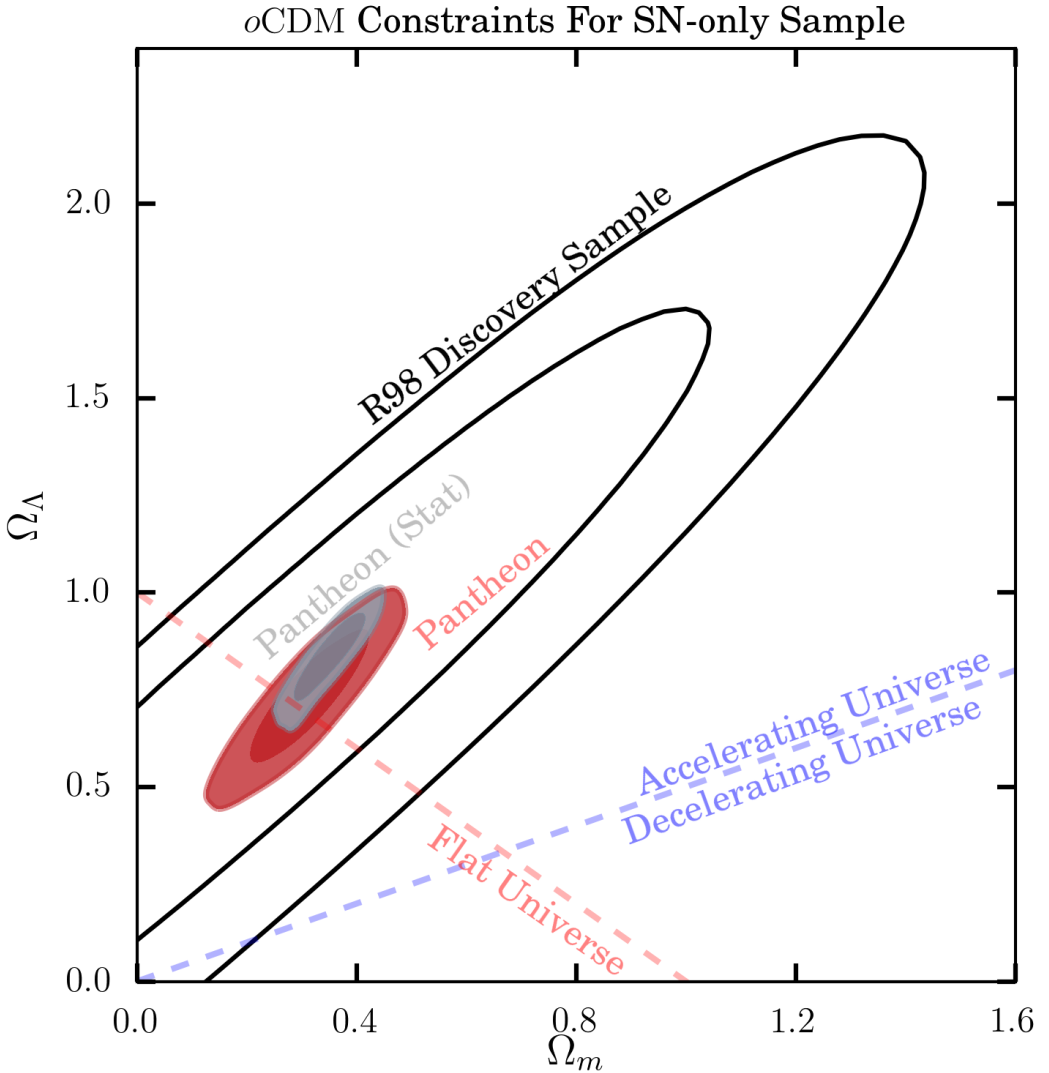
\includegraphics[width=.5\linewidth]{Rapport_figures/scolnic_syst.png}
    \captionsetup{justification=centering}
    \caption{\textit{Contour plot} indiquant la précision à 68 et 90\% de la
    mesure des paramètres $\O_M$ et $\O_\L$ pour la découverte historique de
    \bsc{Riess et. al} (R98, en blanc) se basant sur 100 données de SNe Ia, et
    pour les échantillons actuels utilisant environ 1000 SNe Ia (en rouge). En
    gris est indiqué la part des incertitudes systématiques à l'incertitude
    totale. \cite{scolnic_complete_2018}}
    \label{scolnic_syst}
\end{figure}

Pour continuer à améliorer les mesures cosmologiques, il est donc nécessaire de
travailler sur les sources d'erreurs systématiques, faute de quoi, il sera
impossible d'exploiter l'immense masse de données fournie par LSST. Une des
erreurs dominantes et encore peu étudiée est l'impact de notre connaissance
limitée de la physique des SNe~Ia sur la mesure des paramètres cosmologiques
\cite{rigault_strong_2018} et notamment sur l'évolution potentielle de
$M_B^{\mathrm{corr}}$ en fonction du redshift. La fig~\ref{err_syst} montre une
estimation de l'impact potentiel qu'aurait une évolution réaliste de la physique
des SNe~Ia en fonction du temps sur l'estimation des paramètres ($w$, $w_a$).
Non seulement l'erreur systématique associée est plus grande que la précision
souhaitée pour LSST, mais surtout, la zone mesurée est en désaccord complet avec
ce qui est attendu. La mesure est donc non seulement moins précise, mais elle
est aussi faussée. C'est dans ce cadre que s'inscrit mon stage et la thèse qui
en découle.

\begin{figure}[htbp!]
    \centering
    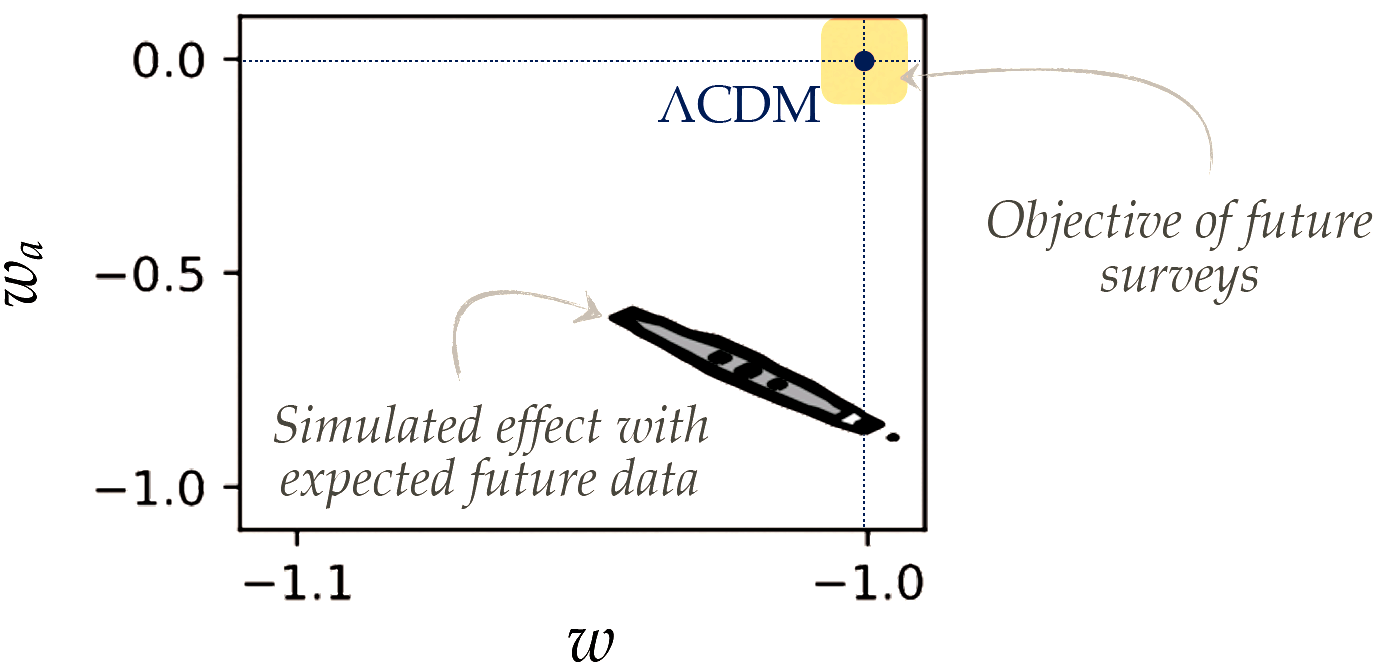
\includegraphics[width=.5\linewidth]{Rapport_figures/error.PNG}
    \captionsetup{justification=centering}
    \caption{Erreur attendue sur la mesure de $w$ et $w_a$ en ne considérant
    que la réduction des erreurs statistiques sans prendre en compte les erreurs
    systématiques.}
    \label{err_syst}
\end{figure}

\section{Construction de l'échantillon d'étude}\label{sec:complet}
\subsection{Évolution de propriétés astrophysiques}\label{ssec:prog}

Un des problèmes majeurs à la réalisation de ce but est que l'on n'a jamais
accès aux supernovae avant qu'elles explosent, sous leur forme de
\textit{progéniteur}, étant donné que les courbes de lumière sont acquises à
partir du moment de l'explosion. Il est donc impossible d'étudier directement
les propriétés des progéniteurs (âge, métallicité...). Pourtant, la physique de
l'explosion à l'origine des SNe Ia dépend de ces propriétés, et on sait que les
propriétés des \textit{étoiles} d'une manière générale évoluent en fonction du
temps ; par exemple, à un redshift de $z \approx 1$, il y avait 40 fois plus de
formation stellaire, et donc de formation de jeunes étoiles. En supposant que
les propriétés des progéniteurs évoluent également avec le temps, et donc avec
$z$, on s'attend à avoir une variation de la magnitude absolue avec le redshift,
ce qui fausserait les mesures du diagramme de Hubble.

\begin{itemize}
    \item Progéniteur inconnus :
    \item L moyennes différentes avec $z$ ou échantillon ;
    \item Évolution du \textit{lsSFR}.
\end{itemize}

Dans la suite de ce rapport, et pour éviter la surcharge de lignes de code, le-a
lecteur-ice pourra se référer aux ressources mises en ligne publiquement sur
\href{https://github.com/Nora-n/variaIa/tree/master/variaIa}{GitHub}
(https://github.com/Nora-n/variaIa/tree/master/variaIa).

\subsection{Effets de sélection}\label{ssec:selec}
La première étape à l'établissement de lois physiques tentant de relier les
variations de magnitudes absolues avec des paramètres mesurable consiste à
travailler sur des données sans effet de sélection qui biaiserait
potentiellement les données recueillies. Or, l'observation du nombre de SNe Ia
analysée en fonction du redshift nous montre l'existence d'un effet de sélection
: en supposant une répartition homogène et isotrope des supernovae dans
l'espace, on s'attend à avoir un nombre de SNe Ia à une certaine distance comme
étant proportionnel au volume de l'espace entre l'observateur et cette distance.
En terme de redshift, on s'attend à la relation $\#\text{SNe Ia} \propto z³$. Si
cette relation est vérifiée jusqu'à une certaine distance, la figure
\ref{redshift_miss} nous montre qu'à partir d'un moment, il n'y a plus de
nouvelles supernovae observées.

\begin{figure}[htbp!]
    \centering
    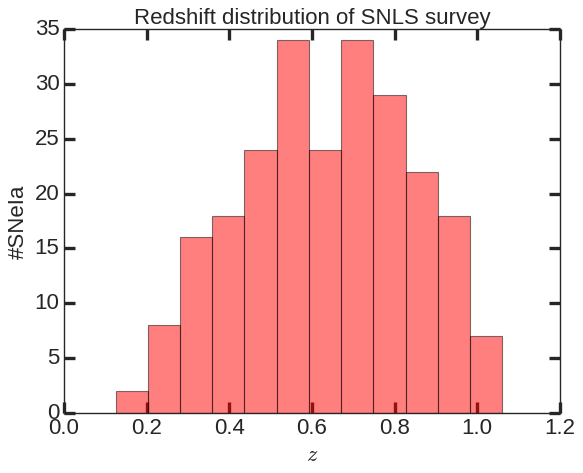
\includegraphics[width=.5\linewidth]{Rapport_figures/redshift_miss.png}
    \captionsetup{justification=centering}
    \caption{Histogramme du nombre de SNe Ia observées en fonction du redshift
    pour les données de l'échantillon SNLS (SuperNova Legacy Survey).}
    \label{redshift_miss}
\end{figure}

Cette évolution est due au fait que notre moyen d'observation des supernovae est
la mesure de flux, comme discuté dans l'introduction (partie \ref{ssec:hub}).
Ainsi, la luminosité totale de la supernova est divisée sur sa surface de
rayonnement, proportionnelle au carré de la distance, et il arrive une distance
où les SNe Ia de luminosités intrinsèques les plus faibles vont être les
premières à ne pas pouvoir être captée par les éléments CCD des instruments de
mesure. Or, comme discuté dans la partie \ref{ssec:lc}, les supernovae de
grandes durées d'explosion sont également plus lumineuses (relation
"brighter-slower"), ce qui veut dire que les supernovae les moins lumineuses
sont également celles de petite durée d'explosion (petit stretch). Le fait de
louper des supernovae à cause d'une luminosité intrinsèque trop faible par
rapport à leur distance à nous n'est donc pas anodin, et il faut s'en prévenir.

\begin{itemize}
    \item Histogramme échantillons ;
    \item Rappel relation \textcolor{red}{brighter-slower} et conclusion.
\end{itemize}

\subsection{Méthode de détermination}\label{ssec:det}
Pour trouver cette distance à partir de laquelle on commence à sélectionner les
supernovae analysées, en l'absence de données précises sur les capacités des
capteurs CCD de chaque échantillon à capter un flux lumineux, l'approche qui a
été choisie repose sur la comparaison entre l'évolution attendue et l'évolution
observée. Comme discuté précédemment, on s'attend à avoir un nombre de
supernovae qui croît proportionnellement à $z³$. En utilisant l'histogramme
précédent, on a, pour chaque intervalle, le nombre de supernovae observées. En
définissant une fonction de paramètre $a$ comme $\#\text{SNe Ia} = a\times
V(z)$, on peut trouver pour chaque milieu d'intervalle le nombre attendu de
supernovae observées selon cette fonction. On peut alors utiliser une
statistique poissonienne pour trouver la probabilité d'avoir ce nombre attendu
sachant qu'on en a effectivement observé le nombre correspondant aux
intervalles. En n'appliquant ce procédé qu'aux premiers intervalles, avant que
le nombre de supernovae diminue par les effets de flux, la correspondance est
bonne, et on peut optimiser le paramètre $a$ en maximisant la probabilité
mentionnée ci-dessus. À partir d'un moment, la correspondance va devenir de
moins en moins bonne et l'optimisation de ce paramètre sera mauvaise. La figure
\ref{zmax_method} est un exemple de ce calcul.

\begin{figure}[htbp!]
    \centering
    \subfigure[7 premiers]{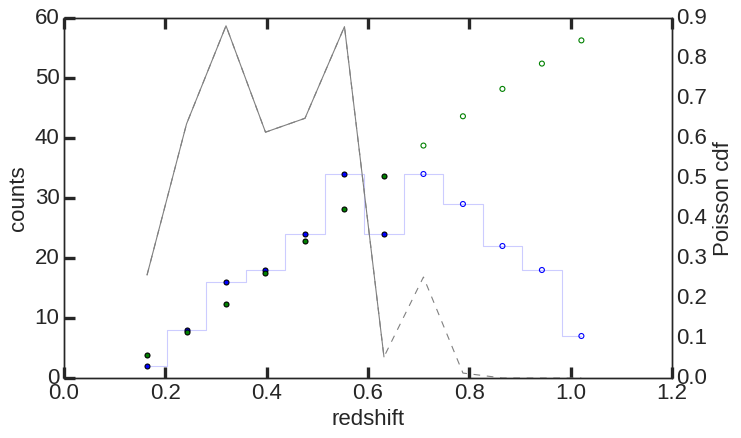
\includegraphics[width=.4\linewidth]{Rapport_figures/zmax_method.png}}
    \subfigure[9 premiers]{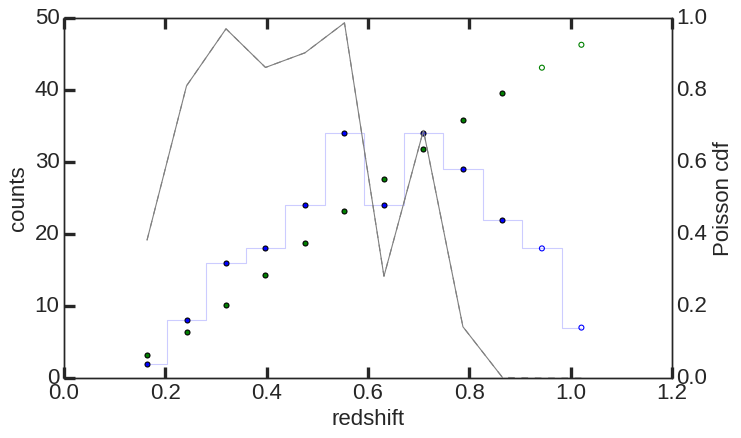
\includegraphics[width=.4\linewidth]{Rapport_figures/zmax_method_2.png}}
    \captionsetup{justification=centering}
    \caption{Graphique présentant l'évolution de la probabilité poissonienne
        d'observer un nombre de supernovae correspondant à la fonction
        $\#\text{SNe Ia} = a\times V(z)$ sachant que l'on en a observé le nombre
        correspondant à l'intervalle. On a ici un exemple pour on n'a considéré
        que les 9 premiers intervalles pour la minimisation, en extrapolant ce
        que cette probabilité deviendrait en prenant plus d'intervalles (en
        pointillés).}
    \label{zmax_method}
\end{figure}

Pour déterminer plus précisément l'intervalle à partir duquel cette probabilité
s'effondre, cette méthode est appliquée 100 fois, avec un histogramme divisé
entre 5 et 13 intervalles de manière aléatoire, où pour chaque itération on
choisit un intervalle maximal aléatoire parmi ces 5 ou 13-là, 4 fois de suite.
Les courbes d'évolution de la probabilité poissonienne sont enregistrées, puis
interpolées linéairement pour finalement en prendre la médiane et l'écart-type.
Le résultat de ce procédé est montré figure \ref{zmax_result}.

\begin{figure}[htbp!]
    \centering
    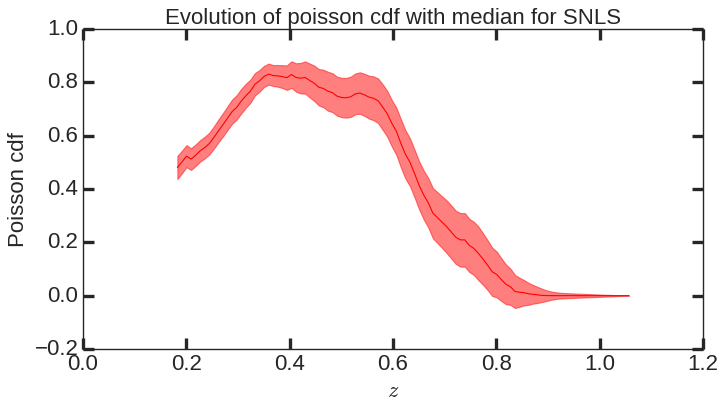
\includegraphics[width=.5\linewidth]{Rapport_figures/zmax_result.png}
    \captionsetup{justification=centering}
    \caption{Résultat du procédé de détermination du redshift maximal à partir
    duquel les effets de sélections ne sont pas anodins.}
    \label{zmax_result}
\end{figure}

On a ainsi déterminé les valeurs maximales de redshifts pour lesquelles ont n'a
pas d'effet de sélection pour les différents échantillons dont on possède les
données. Tous les raisonnements qui suivent s'appuient uniquement sur ces
données dites « complètes », et ce procédé ne sera plus mentionné dans la suite.

\begin{itemize}
    \item Modèle d'évolution ;
    \item Statistique poissonienne, itérations pour chaque échantillon.
\end{itemize}

\section{Modèle d'évolution}\label{sec:stretchevol}
\subsection{Origine du modèle}\label{ssec:stretchevol_ori}

Comme discuté partie \ref{ssec:prog}, le taux de formation stellaire, ci-après
SFR pour \textit{Stellar Formation Rate}, évolue dans le temps. La collaboration
SNF, pour \textit{SuperNova Factory}, a notamment effectué des mesures de
stretch et de taux local spécifique de formation stellaire, LsSFR, c'est-à-dire
le SFR normalisé par la masse stellaire de la galaxie hôte permettant de classer
les galaxies par leur activité stellaire relatives (\textit{spécifique}, sSFR)
dans une distance de $\SI{1}{kpc}$ autour de chaque supernova (\textit{local}).
Il est alors possible de ranger les SNe Ia en deux catégories, celles issues de
progéniteurs vieux au moment de l'explosion et celles issues de progéniteurs
jeunes ; en effet le nombre de jeunes progéniteurs est supposé proportionnel au
SFR qui représente l'activité de formation stellaire, alors que le nombre de
vieux progéniteurs est proportionnel à la masse stellaire de la galaxie hôte
(Mannucci et al. 2005, Scannapieco \& Bildsten 2005), et le rapport des deux
donne, par définition, le sSFR. Le LsSFR est donc un traceur de ce rapport
localement autour des supernovae. Le LsSFR définissant l'âge d'un progéniteur
est choisi de telle sorte à ce qu'il y ait autant de supernovae de chaque sorte,
pour ce redshift-là. Il apparaît alors une corrélation forte entre
le stretch et le LsSFR, comme le montre la figure \ref{snf_data} : on voit qu'on
ne peut pas avoir de supernova vieille avec un grand stretch, ou de supernova
jeune avec un petit stretch.

\begin{figure}[htbp!]
    \centering
    \subfigure[Données brutes]{\label{snf_data}
        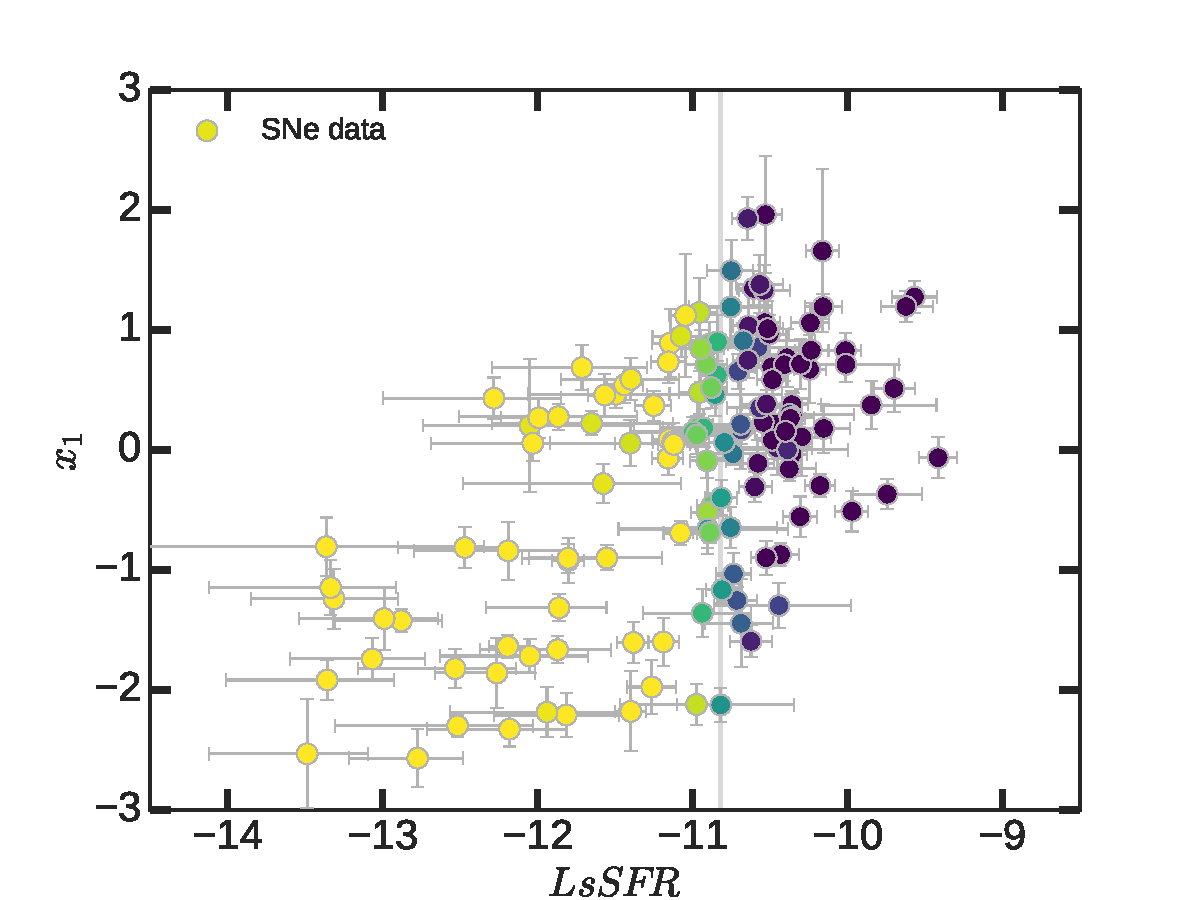
\includegraphics[width=.4\linewidth]{Rapport_figures/BiGaussian_onlydata.pdf}}
    \subfigure[Premier modèle mis en place]{\label{3G2M2S}
        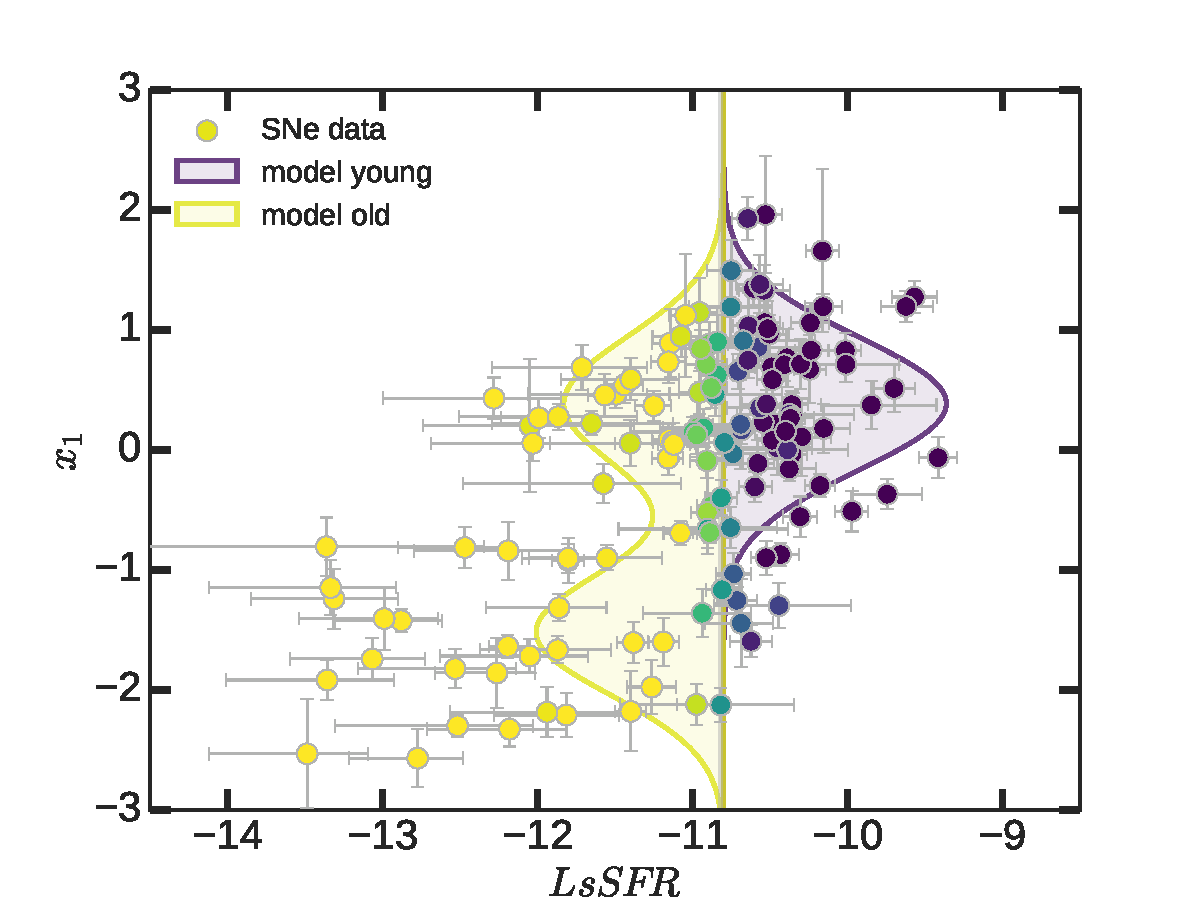
\includegraphics[width=.4\linewidth]{Rapport_figures/BiGaussian.pdf}}
    \captionsetup{justification=centering}
    \caption{Stretch des supernovae étudiées par la collaboration SNF en
    fonction de log(LsSFR). La couleur représente la probabilité pour une
supernova d'être issue d'un jeune progéniteur.}
\end{figure}

On a ainsi essayé de déterminer une loi de distribution du stretch qui puisse
être différente pour les supernovae issues de progéniteurs jeunes ou vieux. Le
premier modèle implémenté est composé d'une distribution gaussienne de moyenne
$\m_1$ et d'écart-type $\s_1$ pour les SNe Ia jeunes, et de la combinaison de
deux distributions gaussiennes pour les SNe Ia vieilles, dont la première est de
même moyenne et écart-type que la première (cf. figure \ref{3G2M2S}).

%\begin{figure}[htbp!]
%    \centering
%    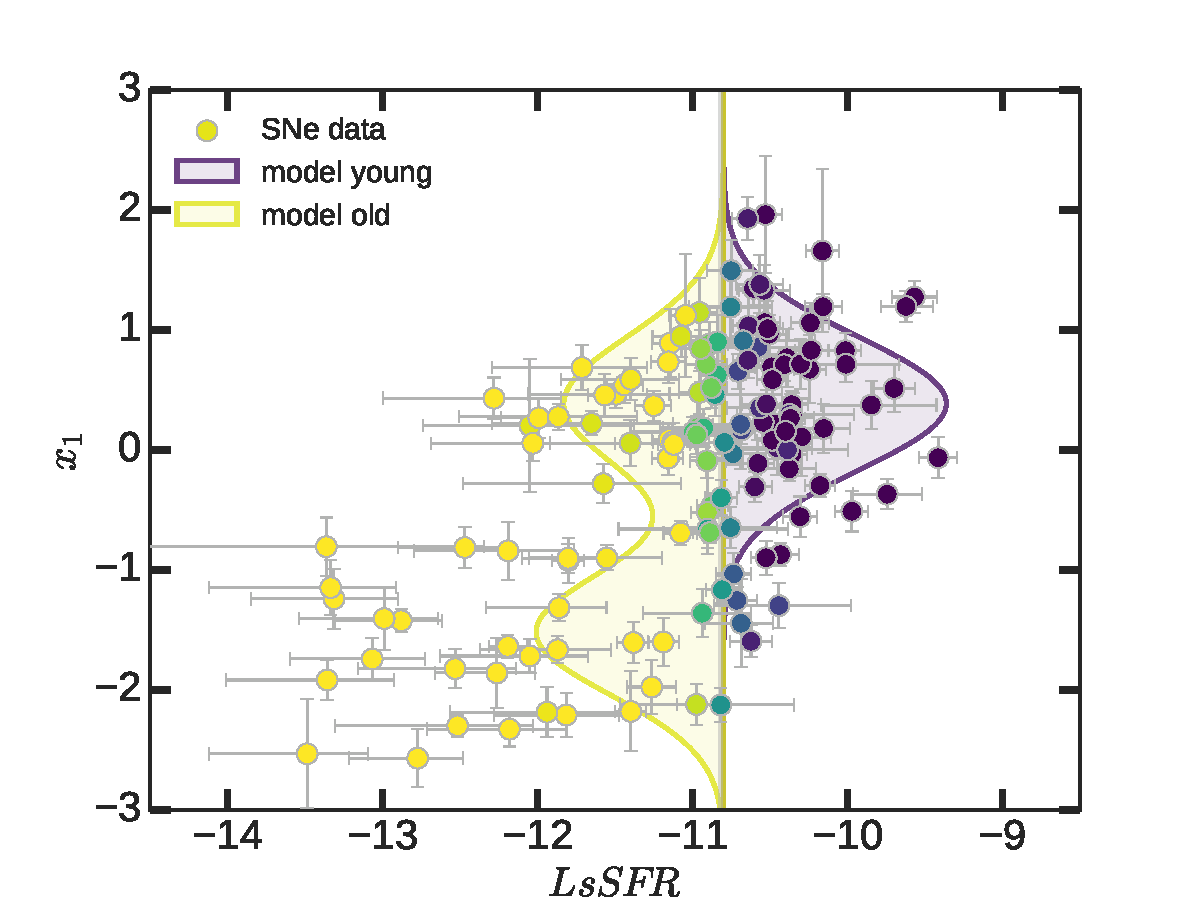
\includegraphics[width=.5\linewidth]{Rapport_figures/BiGaussian.pdf}
%    \captionsetup{justification=centering}
%    \caption{Premier modèle mis en place.}
%    \label{3G2M2S}
%\end{figure}

\begin{itemize}
    \item Données \textcolor{orange}{SNF} ;
    \item Définition jeune/vieille d'après \bsc{Rigault et al.} 2018
\end{itemize}

\subsection{Implémentation aux échantillons}\label{ssec:surveys}
La détermination des données complètes discutée partie \ref{ssec:det} nous a
permis de déterminer le stretch et le redshift moyens des 5 échantillons
étudiés. 
\begin{itemize}
    \item Concordance avec \textcolor{orange}{SNF} seulement
    \item Modèle \textcolor{orange}{SNF} sur toutes les données
\end{itemize}

\subsection{Modifications et comparaisons}
\begin{itemize}
    \item Modification du modèle ;
    \item Implémentation d'autres modèles et résultats
\end{itemize}

\section{Conclusion}
Conclusion.

%\bibliographystyle{aa}
\bibliographystyle{unsrt}
\bibliography{VIDSTIA}
\addcontentsline{toc}{section}{Bibliographie}

\end{document}
